\documentclass[11pt,a4paper]{article}

\usepackage[utf8]{inputenc}
\usepackage[T1]{fontenc}
\usepackage[french]{babel}
\usepackage{graphicx}
\usepackage{geometry}
\usepackage{float}
\usepackage{hyperref}

\geometry{margin=1.5cm}
\setlength{\parindent}{0pt}
\setlength{\parskip}{0.6em}

\title{Atelier 2 - Processus « Recharger son véhicule »}
\author{Maxime MANSIET et Simon GODARD}
\date{12 mai 2026}

\begin{document}

\maketitle

\section*{Objectif}
Ce rendu détaille le cas d'utilisation « Recharger son véhicule » sous forme de diagramme d'activité. Le diagramme présente les actions du conducteur, de la borne, du hub central de la station, de la maison mère et du service de paiement, avec les alternatives entre client inscrit et client anonyme.

\begin{figure}[H]
  \centering
  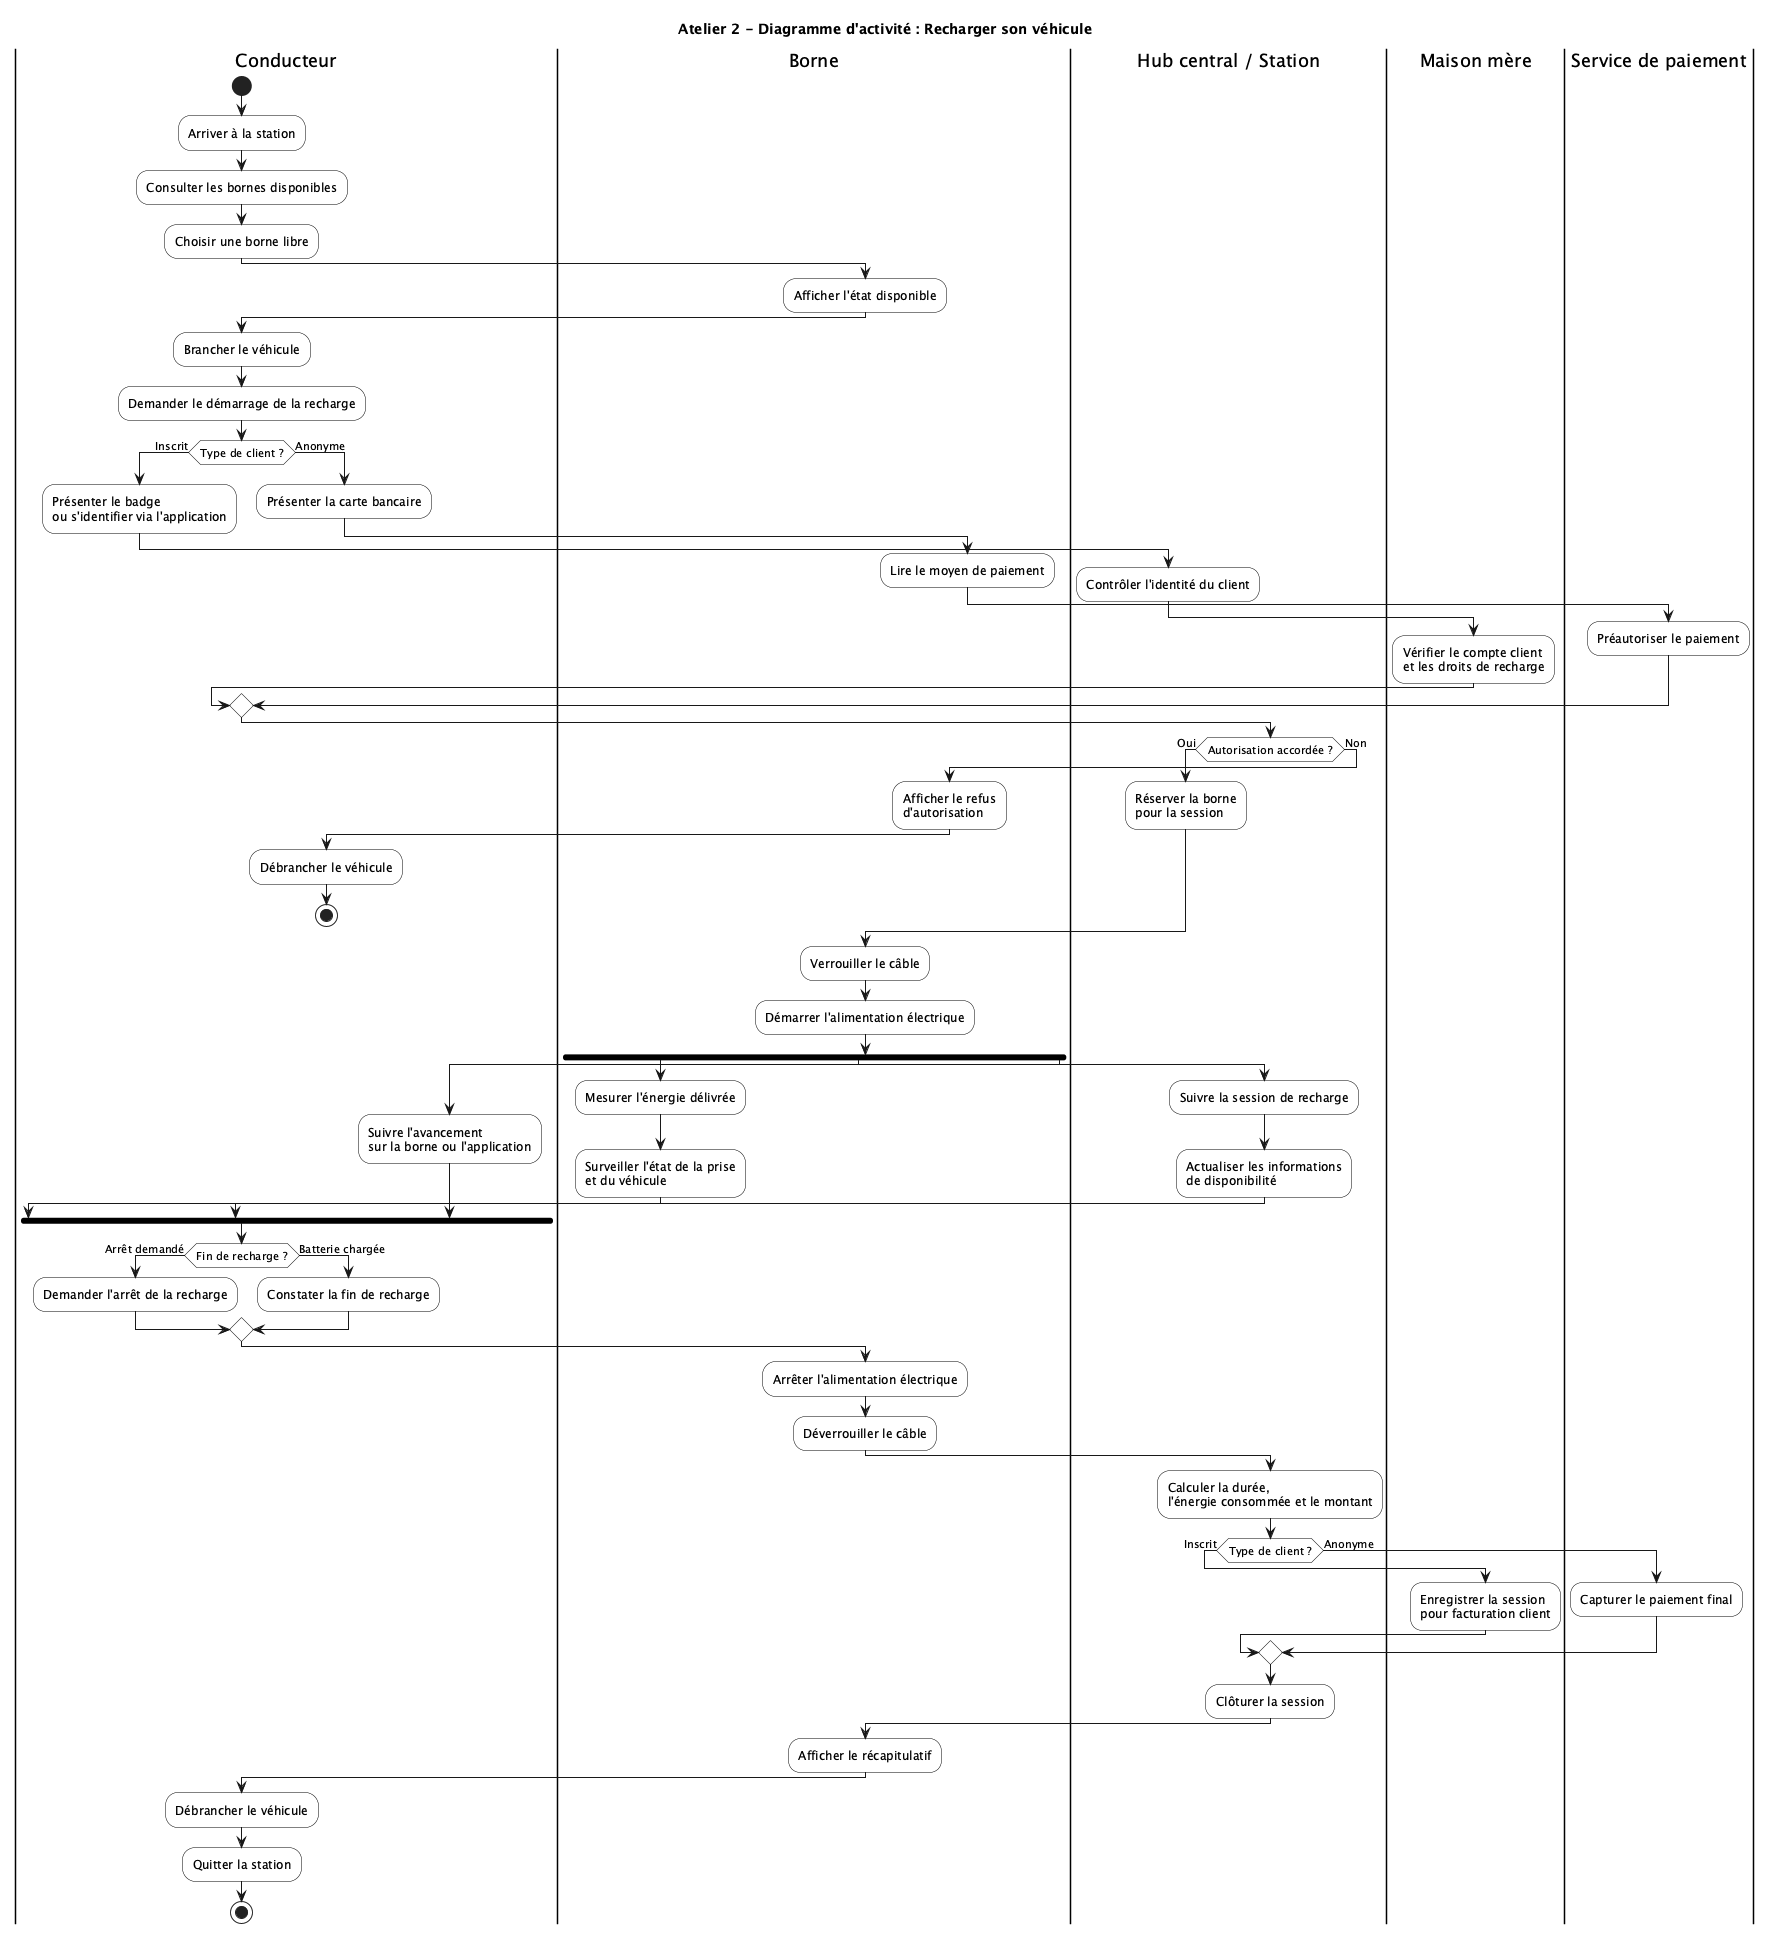
\includegraphics[width=\textwidth,height=0.82\textheight,keepaspectratio]{recharger_vehicule.png}
  \caption{Diagramme d'activité du processus de recharge}
\end{figure}

\end{document}
